\section{Solid 1 - SRP, ISP og DIP}

\subsection{Fokuspunkter}

\begin{itemize}
	\item Redegør for designprincipperne:
	\begin{itemize}
		\item Single Responsibility Principle (SRP).
		\item Interface Segregation Principle (ISP).
		\item Dependency Inversion Principle (DIP).
	\end{itemize}
	\item Redegør for, hvordan du mener anvendelsen af principperne fremmer godt SW design.
	\item Vis et eksempel på anvendelsen af et eller flere af principperne i SW design.
	\item Redegør for konsekvenserne ved anvendelsen af principperne - har det nogle ulemper?
\end{itemize}


\subsection{Single Responsibility Principle (SRP)}
En klasse skal kun have ét ansvar. Derved undgår vi at skulle \textit{rebuild, retest and redeploy} funktionalitet, som ikke er ændret. På samme tid skal det selvfølgelig heller ikke ''overgøres'' sådan at vi får \textit{needless complexity}.\\

''An axis of change is an axis of change, only if changes occur''\\

''Dont apply SRP if there is no symptom''\\

%% side 118 i Agile derp
Modem eksemplet fra side~118 i bogen\footnote{Bogen til kurset: Agile Principles, Patterns, and Practices in C\#}. Skal vi dele modem klassen op? Det kommer an på hvordan applikationen ændrer sig. Hvis connection-delen ændres skal resten af klassen også rekompilere.

\subsubsection{Brud på SRP} \label{sec:brud_isp}
Brud på SRP kan ses på figur~\ref{fig:ISP_bad}~og~\ref{fig:ISP_good} under ISP i section~\ref{sec:isp}. Hvis dette interface har grund til at blive opdelt så er ansvaret muligvis også så anderledes at det burde være i separate klasser.

\subsection{Interface Segregation Principle (ISP)}\label{sec:isp}
\textit{''No client should be forced to depend on methods it doesn't use''}.\\

Når vi har flere klienter som alle bruger samme klasse gennem et interface \textit{IDoThings} som det kan ses på figur~\ref{fig:ISP_bad} vil nogle klienter blive afhængige af metoder som de ikke bruger.

\begin{figure}[H]
	\centering
	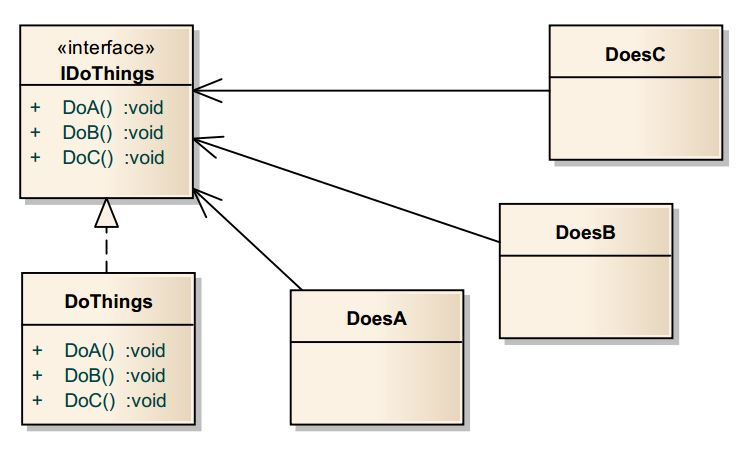
\includegraphics[width=0.7\linewidth]{figs/ISP/ISP_bad}
	\caption{Flere klienter afhængige af samme ''store'' interface.}
	\label{fig:ISP_bad}
\end{figure}

Derfor kan vi ved hjælp af ISP princippet dele interfacet op i flere mindre interfaces. Således undgår vi store og uoverskuelige interfaces, et eksempel er på figur~\ref{fig:ISP_good}.

\begin{figure}[H]
	\centering
	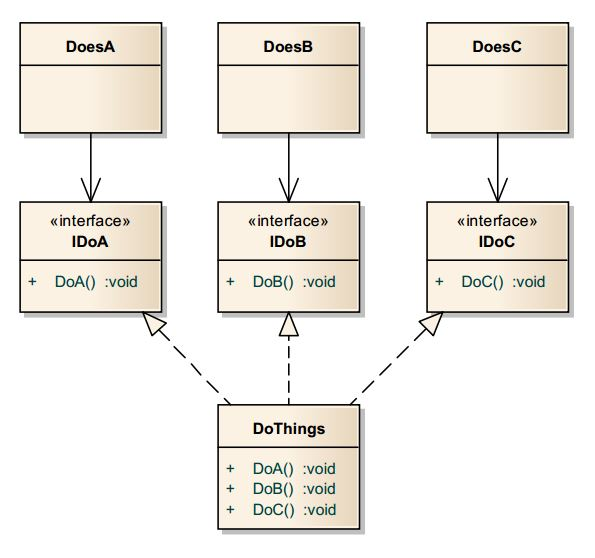
\includegraphics[width=0.7\linewidth]{figs/ISP/ISP_good}
	\caption{ISP anvendt på eksempel fra figur~\ref{fig:ISP_bad}.}
	\label{fig:ISP_good}
\end{figure}

Et eksempel kan være rectangle eksemplet på  \href{http://code.tutsplus.com/tutorials/solid-part-3-liskov-substitution-interface-segregation-principles--net-36710}{denne} side, som også har gode forklaring til de øvrige SOLID principper. Klassen bør ikke indeholde funktion til både draw() og calc(). Dette gør at at fx GUI includen skal bygges samtidig med calc.

Endeligt omkring brud på ISP skal section~\ref{sec:brud_isp} ses på side~\pageref{sec:brud_isp}.

%\subsection{Dependency Inversion Principle (DIP)}
\subsection{Dependency Inversion Principle (DIP)}
DIP har følgende centrale punkter:\\

\textit{''High level modules should not depend on low level modules. Both should depend on abstractions.''}\\

\textit{''Abstractions should not depend upon details. Details should depend upon abstractions.''}\\

Det hedder dependency inversion fordi...\todo{hør fil 1441956 389456 og skriv hvor navnet kommer fra}
\\

Det der menes med abstraktioner her, er interfaces. Et eksempel på DIP er vores øvelse med Compressions Stocking, hvor vi fx havde nogen knapper (high-level) der kaldte noget low-level funktionalitet (blinkende LED’er osv). I stedet for at gøre knappen afhængig af low-level funktionalitetet, lader vi den afhænge af et interface.\\

Klassediagrammet kan ikke være på én side så derfor kan billedet for øvelsen kan ses på  \href{https://raw.githubusercontent.com/BjornNorgaard/I4SWD/bdd4a11a87f182d81b3ed81409a2052e45be82c3/Eksamen/Disposition/figs/compressionstockings_classdiagram.PNG}{dette billede} fra github repo'et.

\subsection{Hvordan fremmes godt SW design?}
Alle tre design principper har deres fordele og nogen, deres ulemper.

\subsubsection{SRP}
At separere klassers ansvar kan være en god ide, idet ethvert ansvar har dets egen ''Axis of change''. Flere ansvar i klasser medfører høj kobling blandt dem. Hvis en enkelt af disse ansvar skal ændres kan det medføre at resten af klassen bliver negativt påvirket eller ''bare'' skal genkompileres, gentestes og genimplementeres.\\

Man skal også passe på ikke at distribuere funktionalitet ud så meget at man får ”needless complexity”. Hvis en klasse ikke har ”brug” for at ændre sig, er der ingen grund til at bruge SRP.\\

Et personligt eksempel \todo{skal med? måske for tidskrævende?} er i faget ISU, hvor vi distribuerede et parkeringssystems funktionalitet ud på enormt mange små klasser, med enkelte metoder/attributter. Dette medførte en meget uoverskuelig og kompleks kode, og det positive ved SRP opvejede ikke længere unødig kompleksitet.

\subsubsection{ISP}

\subsubsection{DIP}

\subsection{Eksempel}
Gode SOLID eksempler på \href{http://blog.gauffin.org/2012/05/11/solid-principles-with-real-world-examples/}{blog.gauffin.org}.

\subsection{Redegør for ulemper}